\section*{ Aplicații cu funcții de ordin superior }

Scopul laboratorului este de a exersa lucrul cu funcții de ordin superior.

\subsection*{ Recapitulare }

O \textbf{funcție de ordin superior} este \textit{o funcție care primește ca argument sau returnează o funcție}.


\begin{tcblisting}{ arc=0pt, outer arc=0pt, listing only, breakable}
applyTwice f x = f (f x)
adder x = (+x)

\end{tcblisting}


\subsubsection*{ Folduri }
Două funcții de ordin superior foarte importante sunt foldurile pe liste: \texttt{foldl} și \texttt{foldr}. Aceasta combină, în mod recursiv, elementele unei liste cu o valoare default, pentru a obține un rezultat.



\begin{tcblisting}{ arc=0pt, outer arc=0pt, listing only, breakable}
foldr (:) [] l         -- intoarce o lista identica cu l
foldl (flip (:)) [] l  -- intoarce inversul listei l

\end{tcblisting}


\begin{tcolorbox}[colback=blue!10, colframe=blue!20]
O variantă importantă a lui \texttt{foldl} este \texttt{foldl'}, care se găsește în modulul \texttt{Data.List}.


\begin{tcblisting}{ arc=0pt, outer arc=0pt, listing only, breakable}
Prelude> import Data.List
Prelude Data.List> :t foldl'
foldl' :: (a -> b -> a) -> a -> [b] -> a

\end{tcblisting}


Puteți citi \texttt{aici} \footnote{\url{https://wiki.haskell.org/Foldr\_Foldl\_Foldl'}} despre diferențele dintre aceste trei folduri.
\end{tcolorbox}

O vizualizare utilă

\begin{figure}[!htb]
\centering
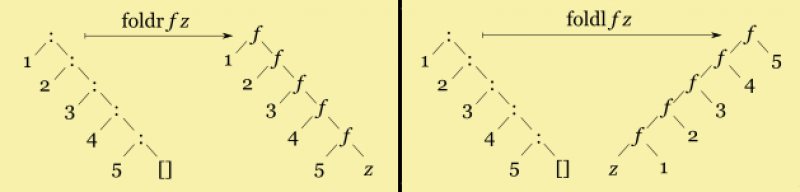
\includegraphics[max width=\textwidth]{:pp:fold-visualization.png}
\end{figure}
:


Tipurile acestor funcții sunt:


\begin{tcblisting}{ arc=0pt, outer arc=0pt, listing only, breakable}
Prelude> :t foldr
foldr :: (a -> b -> b) -> b -> [a] -> b
Prelude> :t foldl
foldl :: (a -> b -> a) -> a -> [b] -> a

\end{tcblisting}


\begin{tcolorbox}[colback=cyan!5, colframe=cyan!10, breakable]
Nu trebie să rețineți pe de rost tipurile. Încercați să înțelegeți ce exprimă și de ce sunt așa.
\end{tcolorbox}

Alte funcții de ordin superior des întâlnite: \texttt{map}, \texttt{filter}, \texttt{zipWith}, \texttt{flip}.


\subsection*{ Exerciții }

1. Fie două matrici reprezentate ca liste de liste. În rezolvarea exercițiilor de mai jos, puteți folosi doar funcții de ordin superior (împreună cu \texttt{take} și \texttt{drop}).

Implementați funcții care să returneze:

\begin{itemize}
	\item  linia \texttt{i} dintr-o matrice
	\item  elementul \texttt{(i, j)} dintr-o matrice
	\item  suma a două matrici
	\item  transpusa unei matrici 
	\item  produsul a două matrici
\end{itemize}


2. O imagine poate fi reprezentată ca o matrice de caractere (numiți, în continuare, "pixeli"). Considerăm că avem trei tipuri de pixeli: \texttt{'.'}, \texttt{'*'}, \texttt{' '}

Implementați următoarele funcții:
\begin{itemize}
	\item  flip orizontal, flip vertical, rotație de 90 în sens trigonometric și invers trigonometric
	\item  negativul (\texttt{'*'} si \texttt{'.'} devin \texttt{' '}, iar \texttt{' '} devine \texttt{'*'})
	\item  scalarea unei imagini cu \texttt{x} unități
	\item  alipirea a două imagini (cu aceeași înălțime) pe orizontală
	\item  alipirea a două imagini (cu aceeași lungime) pe verticală
	\item  crop orizontal de la de la coloana \texttt{x} la coloana \texttt{y}
	\item  crop vertical de la linia \texttt{x} la linia \texttt{y}
	\item  Implementați suprapunerea unei imagini peste o alta (având aceeași dimensiune)
\end{itemize}


\subsection*{ Resurse }

Puteți folosi următoarele pentru a vă testa funcțiile:


\begin{tcblisting}{ arc=0pt, outer arc=0pt, listing only, breakable}
l0="        ***** **            ***** **    "
l1="     ******  ****        ******  ****   "
l2="    **   *  *  ***      **   *  *  ***  "
l3="   *    *  *    ***    *    *  *    *** "
l4="       *  *      **        *  *      ** "
l5="      ** **      **       ** **      ** "
l6="      ** **      **       ** **      ** "
l7="    **** **      *      **** **      *  "
l8="   * *** **     *      * *** **     *   "
l9="      ** *******          ** *******    "
l10="      ** ******           ** ******     "
l11="      ** **               ** **         "
l12="      ** **               ** **         "
l13="      ** **               ** **         "
l14=" **   ** **          **   ** **         "
l15="***   *  *          ***   *  *          "
l16=" ***    *            ***    *           "
l17="  ******              ******            "
l18="    ***                 ***             "

img = [l0,l1,l2,l3,l4,l5,l6,l7,l8,l9,l10,l11,l12,l13,l14,l15,l16,l17,l18]

m1 = [[1, 2, 3], [4, 5, 6], [7, 8, 9]]
m2 = [[1, 0, 0], [0, 1, 1], [1, 0, 1]]

summ1m2 = [[2,2,3],[4,6,7],[8,8,10]]
prodm1m2 = [[4,2,5],[10,5,11],[16,8,17]]

-- functii care printeaza intr-un mod human-readable o matrice sau o imagine
display :: (Show a) => ([a] -> String) -> [[a]] -> IO ()
display displayLine = putStr . foldr (++) "" . map displayLine

-- folositi pentru a afisa o matrice de numere (ex. 1)
displayMat :: (Show a) => [[a]] -> IO ()
displayMat = display (foldr (\x acc -> show x ++ "   " ++ acc) "\n")

-- folositi pentru a afisa o "imagine" - matrice de siruri (ex. 2)
displayImg :: [String] -> IO ()
displayImg = display (++ "\n")


\end{tcblisting}
